%!TEX root = Constructive Alignment for Introductory Programming.tex

\chapter{Guiding Principles} % (fold)
\label{cha:guiding_principles}

%test comment

\graphicspath{{Figures/CAApproach/}}

%
% JG - this is great!
%

This chapter describes twelve principles that underlie our model for delivering constructive aligned introductory programming. These principles act as guidelines for decision making, and in many ways underpin the model as a unit's intended learning outcomes underpin constructively aligned teaching. Each aspect of the model, the associated curriculum, teaching and learning activities, and assessment tasks are aligned with one or more of these principles. 

The principles cover both \emph{how} the teaching and learning environment should operate, and \emph{what} should be taught. Originally derived from constructive alignment, the \emph{how} principles centre on constructivism and aligned curriculum. In relation to \emph{what} should be taught, the principles draw upon computing education literature and our own experiences as educators and software developers. 

Reflective practice played an important part in the formation of these principles, and both sets of principles have developed over the course of this research. This chapter presents the current working principles we use to guide the development and delivery of introductory programming. While most were present throughout the research, their individual emphasis and relationships have developed through our reflective practice. 

%
% JG - I wondered about expanding this to give a bit more overview about what is in each main section??
%

The chapter first outlines the principles related to \emph{how} we aim to teach introductory programming, and then presents the principles related to \emph{what} we aim to teach.


%
% JG - I wonder about "Princiles to guide HOW we should teach"?
%



\section{Principles for how the environment should operate} % (fold)
\label{sub:principles_for_how_the_environment_should_operate}

Interventions that impact on the learning environment, also referred to as the teaching or academic environment, have been shown to have the potential to positively influence student learning outcomes \cite{Trigwell:1991}. Learning environments have also been found to influence students' approach to learning \cite{Entwistle:1990,Entwistle:1991,Kember:2007} and perceptions of teaching environments have been shown to directly, and indirectly, influence learning outcomes \cite{Meyer:1990,Lizzio:2002}. The aim of these first principles was therefore to create a positive learning environment for students; one that is demanding of students but supports and rewards their efforts to understand the concepts being presented. 

The following list outlines these principles for educators:
\begin{enumerate}[noitemsep,nolistsep]
	\item Recognise that students construct knowledge in response to activity. (\Pref{itm:construct})
	\item Align activities and assessment to intended learning outcomes. (\Pref{itm:align})
	\item Assess learning outcomes, not learning pace or product outcomes. (\Pref{itm:formative})
	\item Focus on depth of understanding over breadth of coverage. (\Pref{itm:depth})
	\item Communicate high expectations. (\Pref{itm:expectations})
	\item Actively support student efforts. (\Pref{itm:support})
	\item Trust and empower students to manage their own learning. (\Pref{itm:theory_y})
	\item Be agile and willing to change in response to measurable indicators. (\Pref{itm:agile})
	\item Embed reflective practice in all aspects. (\Pref{itm:reflect})
\end{enumerate}

These first nine principles relate to \emph{how} the teaching and learning environment should operate and could, therefore, be applied to a range of teaching and learning contexts and topic domains.

% \subsection{Relationships between Principles} % (fold)
% \label{ssub:relationships_between_principles}

Individually each principle has its own intrinsic value but intrinsically work together. As a whole, each principle interacts with the other principles to create a productive student centred learning environment.

\begin{figure}[htbp]
	\centering
	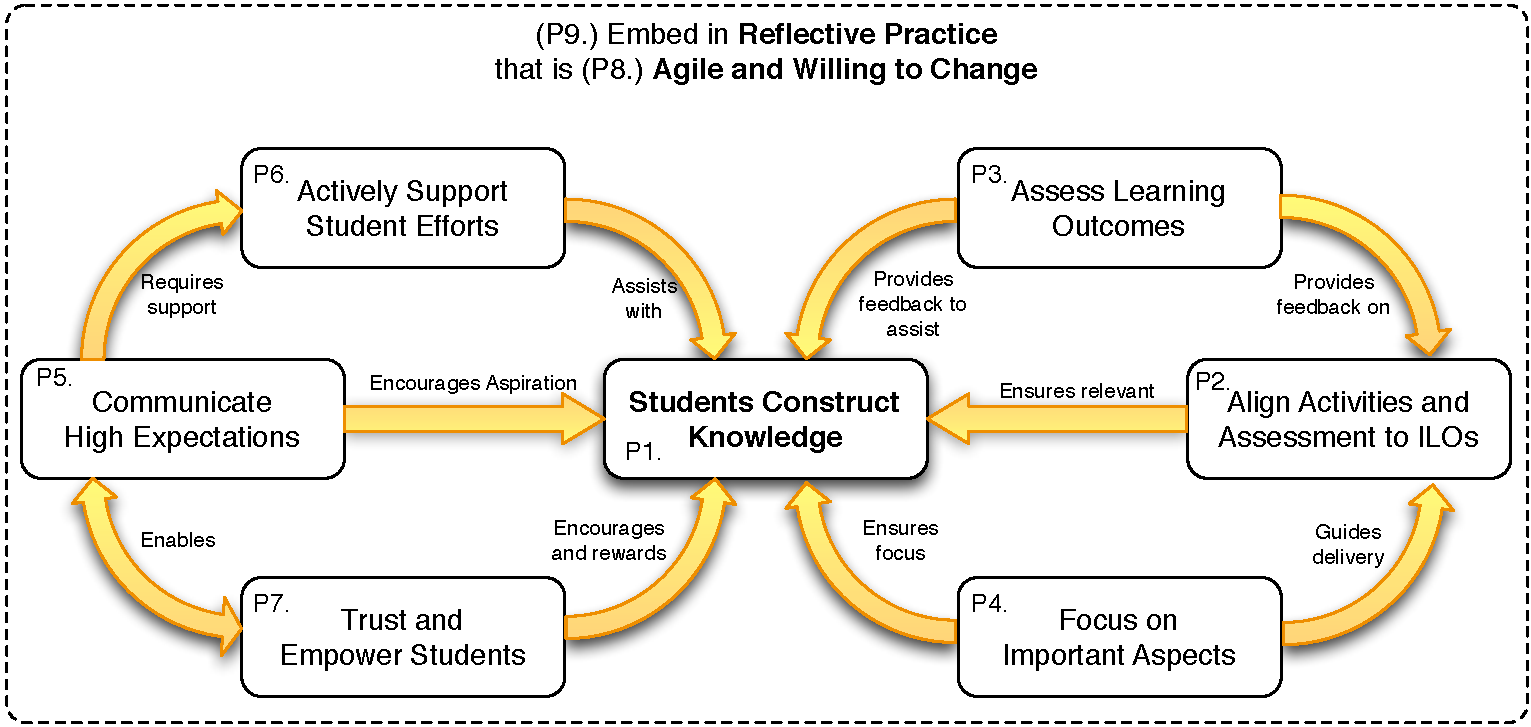
\includegraphics[width=\textwidth]{HowPrinciples}
	\caption{Key interaction between proposed principles for educators.}
	\label{fig:how_principles}
\end{figure}

\fref{fig:how_principles} shows the key interactions between these principles. The students active construction of knowledge is central, with various aspects of this being supported by the other principles. Each principle is discussed in detail in the following sections, with the various relationships being discussed along with associated literature.

% section relationships_between_principles (end)
\bigskip
\subsection{Recognise that students construct knowledge in response to activity} % (fold)
\label{ssub:ideas_adopted_from_constructivism}

Decisions about curriculum, teaching and learning activities and assessment tasks are all guided by the educator's theory of teaching and learning \cite{Argyris:1976,Ramsden:1992}. While constructivism is often promoted by educators, \citet{Phillips:2005} indicates that constructive learning theories have not transitioned to common education practice, resulting in a ``dissonance'' between the elements of effective learning and the characteristics of typical university learning environments. This is symptomatic of the disconnect between educators espoused theory and their theory-in-use \cite{Argyris:1976}. To successfully implement constructive alignment it is, therefore, important to adopt the key aspects from constructivism outlined by \citet{Biggs:1996c}, \citet{Biggs:1997} and in \citet{Biggs:2007}. By adopting constructivism as our theory-in-use we aimed to create an educational setting that was ``in harmony'' with the principles of constructive alignment.

Central to all forms of constructivism is the principle that \emph{learning is an active process requiring the leaner to construct their own understanding through individual and social activity} \cite{Biggs:1996c,Duffy:1996,Duffy:1992,Glasersfeld:1989,Steffe:1995}. 

%
% JG - could add appropriate citations for source of each of these, if different
%

The following aspects of constructivism are actively embedded in the model presented in the next chapter:
\begin{itemize}[noitemsep,nolistsep]
	\item Knowledge is constructed, not transmitted via communication alone.
	\item Teaching involves creating a context in which learners are able to construct appropriate cognitive models through individual and social activities \cite{Cobb:1994}.
	\item Errors in understanding are opportunities for further learning, as these help indicate the students' current level of development and can be used to guide future learning activities.
\end{itemize}

\citet{Biggs:1996c} reason for adopting constructivism as a central philosophy was due to its emphasis on the students active role in constructing their own knowledge. When taken to an extreme this can result in approaches that rely upon students building their own understanding from ``first'' principles, isolated concepts and without structure. Such approaches are often promoted in discovery learning \cite{Bruner:1961} and are often promoted in constructivist writings, such as in \citet{Glasersfeld:1989} and \citet{Duffy:1996}. The unstructured nature of these teaching and learning environments have received strong criticism. \citet{Anderson:1998} criticises constructive learning theories when ``pursued to unproductive extremes'', as in the case with discovery learning. \citet{Mayer:2004} argues against discovery learning, instead suggesting that constructivist views of education may be better served through cognitive activity, instructional guidance, and curricular focus. Furthermore, \citet{Kirschner:2006} argue against discovery learning indicating that in highly complex environment, such as with software development, free exploration may generate a heavy workload and detrimentally affect learning. 

%
% JG -  this reads a tad forward referencing to "the model" - could rephrase/retense to present e.g.
% "requires"  and "This approach will temper..."
%
% Presumabely many of these principles could be applied to produce a different model?
%

Embedding constructivism in the model required accepting the central role of the learner in constructing their knowledge, while avoiding detrimental aspects associated with taking these ideas to their extreme. The result was to temper constructivism with certain practical details, an approach we feel is in line with the principles of constructive alignment as originally proposed by \citet{Biggs:1996c}. These details include the following:

\begin{itemize}[noitemsep,nolistsep]
	\item Communication remains a valuable tool for educators to help shape the learning context.
	\item Guided instruction is valuable and ensures student activity is likely to be productive.
	\item Deliberate practice provides students with opportunities to engage with principles in action.
\end{itemize}

% section ideas_adopted_from_constructivism (end)

\subsection{Align activities and assessment to intended learning outcomes} % (fold)
\label{ssub:align_activities_and_assessment_to_intended_learning_outcomes_}

In order to implement constructive alignment we need to work iteratively toward achieving a ``web of consistency'' \cite{Biggs:1999} in which we optimise the likelihood of students \emph{engaging appropriately} with learning activities and assessment tasks. \cite{Biggs:1996c} indicates that this can be achieved through aligning learning activities and assessment tasks to the unit's intended learning outcomes. 

The alignment of activities and assessment to intended learning outcomes is critical for our model. As shown in \fref{fig:how_principles}, this alignment is seen as supporting student construction of knowledge. By aligning teaching and learning activities to the intended learning outcomes we ensure that students are constructing the required understanding. Similarly, by aligning assessment with these same intended learning outcomes we ensure that students are adequately prepared for this assessment and that the assessment is evaluating students' attainment of the stated learning outcomes. 

One potential issue identified in \cref{cha:background} is relying too heavily on staff to perform this alignment. Where students are not involved, there are additional opportunities for misalignment. \fref{fig:alignment} is an altered version of \fref{fig:misalignment} from \cref{cha:background}. \fref{fig:misalignment} was used to highlight the opportunities for misalignment as the intended learning outcomes sat outside the process, interacted with only by staff in designing the assessment tasks. 

\begin{figure}[htbp]
	\centering
	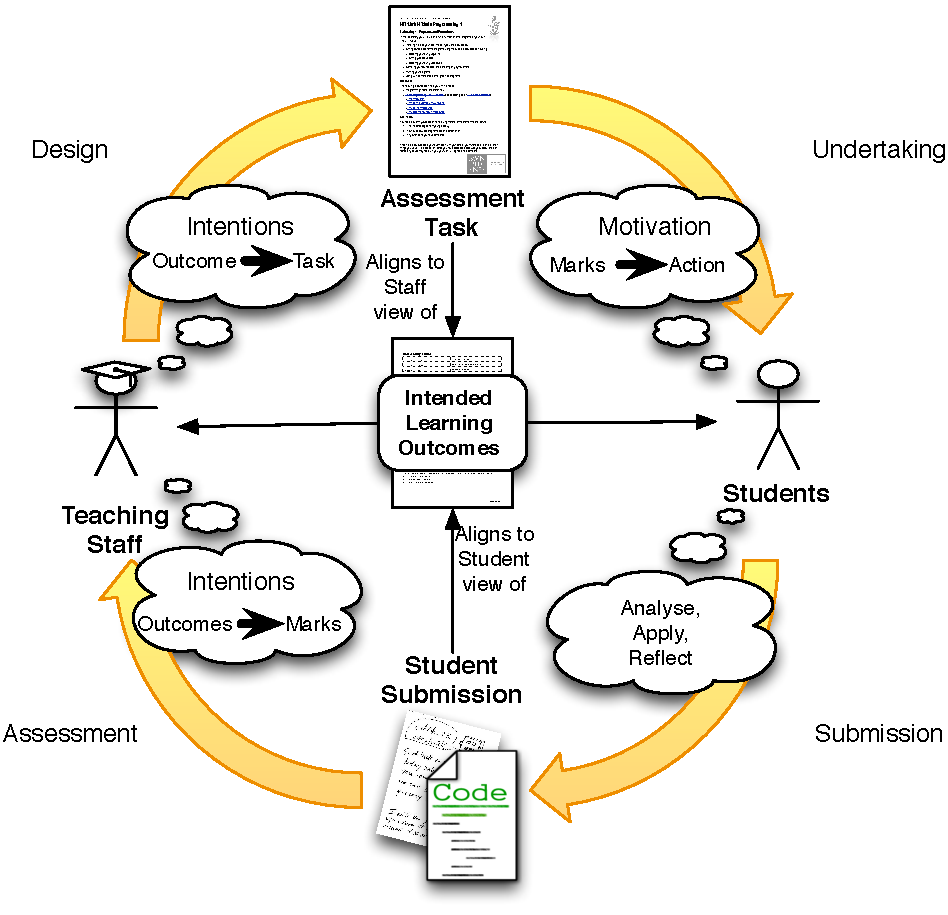
\includegraphics[width=\textwidth]{Alignment}
	\caption{An altered version of \fref{fig:misalignment} with students and staff now actively involved in aligning work to the unit's intended learning outcomes}
	\label{fig:alignment}
\end{figure}

The intended learning outcomes become central to this process when students must also align their work with these outcomes, as shown in \fref{fig:alignment}. Opportunities for misalignment are still possible, and therefore iterative improvements will still be required, but the process is now more focused on the stated intended learning outcomes. Staff and students now need to develop a shared understanding of the intended learning outcomes, and collaboratively work toward students being able to demonstrate they have met all outcomes. In this way, it should be possible to achieve the ``web of consistency'', and hopefully thereby improve the chances that students engage appropriately with learning activities and assessment tasks. 

% subsection align_activities_and_assessment_to_intended_learning_outcomes_ (end)


\subsection{Assess learning outcomes, not learning pace or product outcomes} % (fold)
\label{ssub:aim_to_assess_learning_outcomes_not_learning_pace_or_product_outcomes_}

Assessment in education is often seen as serving one of two purposes: supporting learning, or evaluating outcomes. These two purposes are known as \emph{formative assessment} and \emph{summative assessment}, as proposed by \citet{Scriven:1967} and \citet{Bloom:1969}. Formative assessment aims to assess student learning for the purpose of providing \emph{feedback}. This is distinct from summative assessment where the aim is to assess how well students have perfomed on a certain task, typically to determine a final \emph{grade}. \citet{Biggs:2007} suggest that the two forms of assessment are better referred to as \emph{formative feedback} and \emph{summative grading}.

The important role of formative feedback in education is widely reported. \citet{Ramsden:1992} indicates that of all items on the Course Evaluation Questionnaire \cite{Ramsden:1991} the one that most clearly distinguished between the best and worst courses related to the provision of helpful feedback. \citet{William:2006} described the use of formative feedback in short, medium and long cycles to improve student learning, and indicated that to be formative outcomes of the assessment must be used make adjustments to better meet students' learning needs. \citet{Black:1998} show that substantial learning gains can be achieved by innovations designed to strengthen frequent feedback students receive. Furthermore, \citet{Black:1998} report that students pay more careful attention to feedback when there are no associated marks. In discussing assessment for learning \citet{Brown:2004} stated that ``Formative feedback is critical'' and that ``feedback must be at the heart of the process'' if we are to make assessment an integral part of learning. 

\citet{Gibbs:2004} listed ten conditions under which assessment assists with student learning. These ten conditions can be summarised into three main points: 

%
% JG - are these all in your own language/paraphrased - if so, good.  If not, reword :-)
%

\begin{itemize}[noitemsep,nolistsep]
	\item Assessment tasks are aligned with intended learning outcomes, and provide students with sufficient work to ensure they engage appropriately with the required learning.
	\begin{enumerate}[noitemsep,nolistsep]
		\item Sufficient assessed tasks are provided for students to capture sufficient study time.
		\item These tasks are engaged with by students, orienting them to allocate appropriate amounts of time and effort to the most important aspects of the course.
		\item Tackling the assessed task engages students in productive learning activity of an appropriate kind.
	\end{enumerate}
	\item Feedback is constructive in nature, providing information that students will be able to use to develop.
	\begin{enumerate}[noitemsep,nolistsep,start=4]
		\item Sufficient feedback is provided, both often enough and in enough detail.
		\item The feedback focuses on students' performance, on their learning and on actions under the students' control, rather than on the students themselves and on their characteristics.
		\item The feedback is timely in that it is received by students while it still matters to them and in time for them to pay attention to further learning or receive further assistance.
		\item Feedback is appropriate to the purpose of the assignment and to its criteria for success.
		\item Feedback is appropriate, in relation to students' understanding of what they are supposed to be doing.
	\end{enumerate}
	\item Students utilise the feedback.
	\begin{enumerate}[noitemsep,nolistsep,start=9]
		\item Feedback is received and attended to.
		\item Feedback is acted upon by the student.
	\end{enumerate}
\end{itemize}

% \citet{Mattick:2007} identified the perceived lack of feedback as a barrier to creating a high quality learning environment for undergraduate medical students. 

The experience of \citet{Smith:2005} indicates that shifting to formative assessment requires more than simply removing summative marks. \citet{Smith:2005} reported significantly worse results for the group of early secondary student who received only formative feedback. In discussing their results, they indicate that in this case feedback comments were not often constructive, were misunderstood by students, and were not integrated back into the teaching and learning context. It appears that in the case examined by \citet{Smith:2005} the assessment remained primarily summative in nature with marks being replaced by comments, resulting in many of the conditions raised by \citet{Gibbs:2004} had not been met.

In proposing the use of formative assessment in education, \citet{Bloom:1969} indicates that an assessment item can play both formative and summative roles, though he suggested that in this case the formative assessment will be less effective. The issue with this is that the purpose behind the two forms of assessment will result in students approaching these in different ways. To make the most of formative feedback the ideal strategy for students is to highlight their misunderstandings, drawing attention to what they do not know. By doing this, students will receive feedback that is more relevant to their current situation and will provide them with the advice they need to make progress. In contrast, misunderstandings result in lower grades when the assessment is summative. As a result, summative grading encourages students to hide their misunderstandings. In extreme cases students plagiarise others work in an attempt to hide their own misunderstandings, something that does not make sense when the work is formative in nature. 

\fref{fig:pace} highlights another issue with the use of summative assessment during the teaching period. This figure shows three hypothetical students, Student ``A'', Student ``B'' and Student ``C'', and their depth of understanding over the teaching period. At the start of the teaching period each comes in with existing knowledge, and during the teaching period they construct additional knowledge. When assessment 1 is performed each has achieved some level of understanding that is compared against an expected level of achievement. When summative grading is used at this point Student ``C'' has not made sufficient progress and would receive a low grade: they have learnt too little. At the same time Student ``A'' has not been pushed by this assessment, and there is little recognition for this students advanced understanding: they have learnt too much. Student ``B'' is somewhere between these two, and therefore receives a ``good'' grade: they have learnt just enough. The first assessment is punishing Student ``C'' for learning these topics too slowly, and is discouraging Student ``A'' by not recognising their current level of understanding.

\begin{figure}[p]
	\centering
	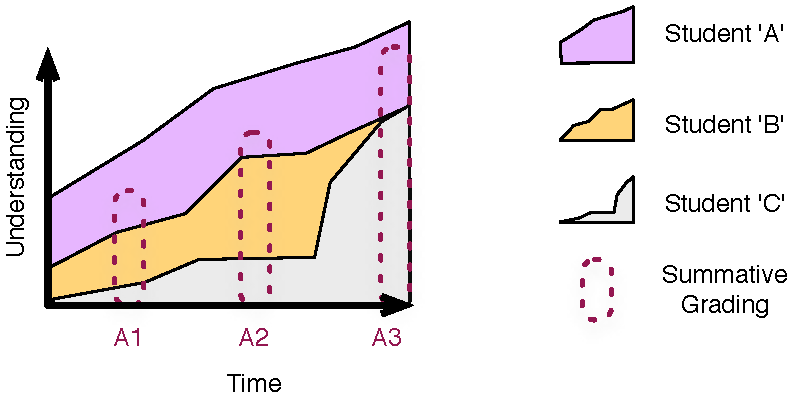
\includegraphics[width=0.75\textwidth]{PaceOfLearning}
	\caption{A hypothetical scenario, showing summative grading measuring pace of learning.}
	\label{fig:pace}
\end{figure}

\begin{figure}[p]
	\centering
	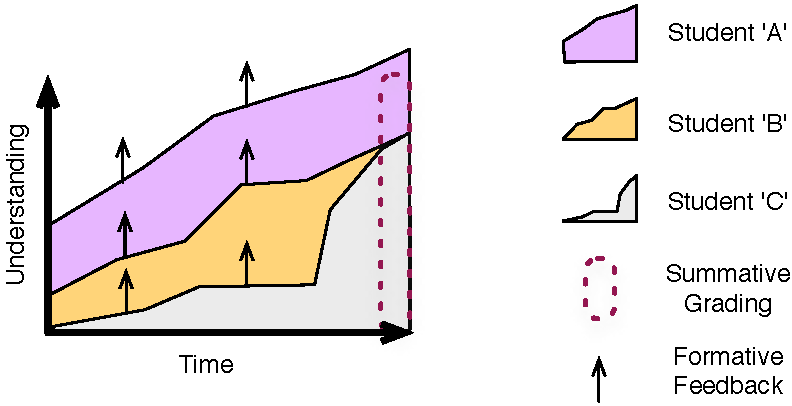
\includegraphics[width=0.75\textwidth]{FormativeFeedback}
	\caption{An alternative to \fref{fig:pace}, showing formative feedback supporting learning during delivery with summative grading at the end.}
	\label{fig:formative}
\end{figure}

Similar patterns occur for the second assessment later in the teaching period. Student ``A'' is still not begin challenged, Student ``B'' is progressing nicely, and Student ``C'' is struggling. For Student ``C'' this negative reinforcement may possibly discourage them from attempting to master the concepts, and reinforce any negative opinion they have of the field in general. In this case, however, Student ``C'' more fully grasps the concepts after the completion of the second assessment. The concepts start to come together, and by the end of the unit Student ``B'' and Student ``C'' have a comparable depth of understanding. This result will, however, not be reflected in their results. Given that each of the assessment items in our hypothetical unit were summative, Student ``C'' will have lost significant marks from the first two assessment items. In effect, the summative assessment is not only assessing the final level of understanding, but also the pace at which the student was able to achieve this understanding. 

%
% JG - "no" -> "not"?
%

This grading during the semester is also no effective for the high achieving Student ``A''. At no point has their advanced knowledge been recognised, and the constrained nature of the assessments are not likely to have helped their development. 

\fref{fig:formative} shows an alternative picture, one that makes use of formative feedback and delays all summative assessment to the end of the teaching period. At each of the assessment points during the semester the students each receive formative feedback based on the level of understanding they demonstrate at that point. The advanced standing of Student ``A'' can be recognised, and the student can be encouraged to further their understanding with additional resources and advice. Student ``B'' can be congratulated for making good progress, their misunderstandings can be addressed and they can be advised how best to proceed with the upcoming material. Student ``C'' can be offered additional support or directed to useful resources, their lack of progress is not punished but used to indicate the student needs additional help. This more personal help and attention should result in improved learning, but even when the progress remains the same the summative assessment at the end of the semester is still a better representation of the students' learning outcomes.

%
% JG - I suggest move 3.3 to here
%

\bigskip

To best support student construction of knowledge the model presented in the next chapter aims to maximise the use of formative assessment: assessment that supports learning. This involves the use of frequent formative feedback during the semester to aid students in developing appropriate understanding, and delaying summative assessment until after unit delivery.

Our assessment should, as much as possible, focus on providing feedback on student understanding and ability to meet the intended learning outcomes. We want to focus on more than just the ``product'' outcomes from the teaching and learning activities. Assessment tasks need to include aspects that require students to articulate their current understanding of concepts. This can then be used to help determine the students current level of understanding, and errors evident in this work provides opportunities for students to learn from their mistakes. 

This principle relates to both students construction of knowledge and to the alignment of activities and assessment, as shown in \fref{fig:how_principles}. Formative assessment of learning outcomes during delivery helps students in the construction of knowledge, providing opportunities to learn from their mistakes without fear of losing marks. These formative tasks also help both staff and students with the alignment of teaching and learning activities and assessment tasks. Staff can use the identified misunderstandings to help guide students individually, and to change or adjust teaching and learning activities where needed. For students, this ongoing focus on articulation of understanding and receiving feedback will ensure they are suitably prepared to demonstrate how they have met all of the intended learning outcomes in the final summative assessment.

The summative assessment also contributes to both students construction of knowledge and to the alignment of activities and assessment. For final unit grades students will need to demonstrate how their understanding aligns with the units intended learning outcomes. The assessment needs then to aim to assess the level of understanding demonstrated, in effect aiming to evaluate how suitable the students level of understanding is at the end of the unit. The SOLO taxonomy (Structure of the Observed Learning Outcome) proposed by \citet{Biggs:1982} provides effective guidelines for performing such an assessment.

To summarise, the model presented in \cref{cha:approach} aims to enhance learning outcomes through the use of frequent formative feedback. This will aim to meet the requirements from \citet{Gibbs:2004}, thereby avoiding the issues raised by \citet{Smith:2005}. To be effective, the formative feedback must be communicated effectively to students and provide them with clear means of addressing any shortcomings.

% subsection aim_to_assess_learning_outcomes_not_learning_pace_or_product_outcomes_ (end)

\subsection{Focus on depth of understanding over breadth of coverage} % (fold)
\label{ssub:focus_on_depth_of_understanding_over_breadth_of_coverage_}

With limited resources, primarily time, the classic depth-vs-breadth trade off needs to be considered. Given that we have fixed time, we can either focus on providing a breadth of coverage or a depth of understanding, as illustrated in \fref{fig:depth}. 

\begin{figure}[htbp]
	\centering
	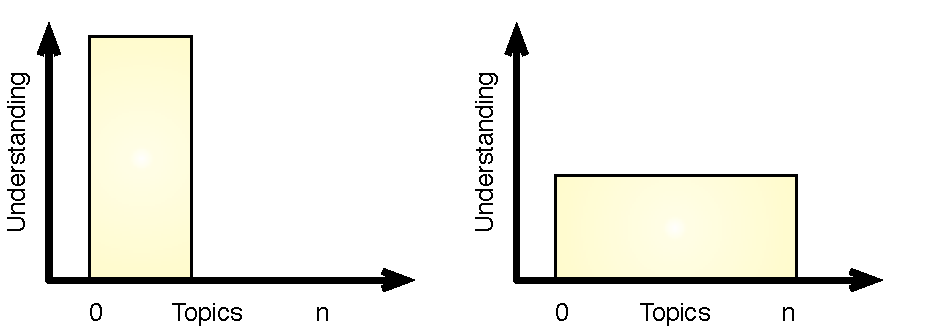
\includegraphics[width=0.75\textwidth]{DepthOrBreadth}
	\caption{Given a fixed teaching ``volume'', a unit can cover either a breadth of topics or fewer topics in depth.}
	\label{fig:depth}
\end{figure}

%
% JG - are there other studies supporting this that can be cited??
%


The study conducted by \citet{Schwartz:2009} found that high school students who reported studying a major topic in depth earned higher grades in college than those who reported covering no topics in depth. If this can translate to undergraduate computing education, then a depth of understanding in programming may help students succeed with other computing units. Given the strong correlation generally observed between programming skills and other computing skills \cite{McGettrick:2005} this is likely.

This principle also extends beyond topic selection, permeating every aspect of the delivery. In communicating concepts it is important to focus on only core aspects, ignoring interesting but unnecessary details. We want to aim to have as high a signal to noise ratio \cite{Shannon:1949} as possible, ensuring students will not miss important details amongst the noise.

As programming is central to the discipline of computing \cite{McGettrick:2005} it will be important to focus on building depth of understanding, over covering a breadth of topics. This is particularly challenging as external parties seek to inject more content into curriculum. There is a constant pressure to include details on contemporary topics such as developing for mobile devices, web application programming, building graphical user interfaces, using certain programming languages, development environments, or software tools. Introducing such topics may have some merit, but runs the risk of inappropriately focusing students attention. A successful introductory unit should focus on building sufficient depth of understanding such that that these additional topics could be learnt by the student on their own. Where a breadth approach is taken students may learn contemporary tools at the risk of missing the underlying concepts that would enable them to move beyond what they have learnt.

Depth over breadth will help focus the teaching and learning activities and assessment tasks, and ensure that they align to sufficiently deep cognitive levels. As the tasks define what students will do, this will in turn help ensure that students are developing appropriately deep knowledge in relation to the intended learning outcomes.

% subsection focus_on_depth_of_understanding_over_breadth_of_coverage_ (end)

\subsection{Communicate high expectations} % (fold)
\label{ssub:have_high_expectations_of_students_}

Communicating high expectations was an important part in the development of the model. In listing their principles for good undergraduate education, \citet{Chickering:1987} include communicating high expectations as one of their seven principles. \citet{Chickering:1987} state ``expect more and you will get more'' and indicate that high expectations are important for everyone, from those who are poorly prepared or unwilling to exert themselves to those who are bright and motivated. Similarly, \citet{Klem:2004} reported that elementary and secondary school students were likely to be more engaged with learning if they perceived their teachers as using a well structured environment with high expectations. 

Believing in students' potential is also key to the approach presented by \citet{Soetanto:2003,Soetanto:2012}. Soetanto's approach aims to improving students' discipline, confidence and belief in their potential, and units delivered with this approach have gained in popularity despite their technical difficulty and being delivery in a foreign language (English). 

By having high expectations of our students we aim to build student confidence and get them to aspire to excellence. These expectations will then require students to work hard throughout the unit's delivery, providing encouragement to spend sufficient time on the teaching and learning activities. This then required both time and energy from students, which should improve outcomes: as stated by \citet{Chickering:1987} ``time plus energy equals learning''.

% subsection have_high_expectations_of_students_ (end)

\subsection{Actively support student efforts} % (fold)
\label{ssub:actively_support_student_efforts}

Both \citet{Chickering:1987} and \citet{Soetanto:2003,Soetanto:2012} indicate high expectations should also apply to teaching staff. If the students are to meet our high expectations, they will need our active support. This will need to extend beyond providing formative feedback, to providing active support throughout the process. Given the technical nature of introductory programming and the exacting nature of compiler, students are going to face numerous challenges.

This requires the recognition of student differences, and preferred learning styles. The various works on learning styles \cite{Coffield:2004} indicate that individuals have different preferences with how they approach their learning. By providing support for a range of learning approaches, and through using different ways of communicating the same ideas, the model helps students in the construction of their knowledge. Enabling them to approach concepts and topic from a variety of angles.

% subsection actively_support_student_efforts (end)

\subsection{Trust and empower students to control their own learning} % (fold)
\label{ssub:trust_and_empower_students_to_control_their_own_learning}

%
% JG - I think this is very nice discussion :-)
%


Student motivation has a significant impact on learning. In terms of strategies for improving student motivation, McGregor's work on motivational strategies in business provide some insights into similar strategies that could be applied to education \cite{McGregor:1960}.  In his work on personnel management, McGregor identified two means of categorising how managers perceived their employees: named ``Theory X'' and ``Theory Y''. Traditionally businesses were seen to use coercion or persuasion as a strategy to motivate employees to achieve required levels of productivity. These strategies are used when managers adopt the view that employees do not want to work and cannot be trusted, \citet{McGregor:1960} named this understanding of human motivation as Theory X. In contrast, Theory Y assumes that, given the right conditions, people want to work, that they can be trusted and will do their best work when they are.

While originally applied to business organisation management, these views can also be applied to an educational setting. \citet{Markwell:2004} categorised Theory X and Theory Y positions for educational settings, as outlined in \tref{tbl:theoryx_y}. In the educational context, Theory X is dominated by a negative view of students and their motivation. Staff are central to the distribution of knowledge, and students must be coerced into learning. The role of the teacher is seen more as a \emph{sage on a stage}. These attitudes are unlikely to lead to student centred approaches to learning, and grate against constructivist thinking.

The contrasting Theory Y position takes a more positive view of students, their potentials and willingness to learn. Students are viewed as being naturally inquisitive, willing to learning, and capable of engaging appropriately with the learning activities. The role of the teacher is seen more as a \emph{guide by the side}. The resulting teaching and learning context is likely to lead to student centred approaches that are more in keeping with constructivist thinking.

These two perspectives represents the two extremes, and no one individual is likely to hold a pure Theory X or Theory Y position. \citet{Markwell:2004} differentiated between a Hard and Soft form of Theory X. Hard Theory X teachers focus on the punitive aspects of the assessment, focusing on the punishments for not following the rules. While Soft Theory X uses marks for encouragement, with the use of bonus marks or similar motivations. In contrast, Theory Y focuses on providing opportunities and resources for students to learn from.

In order to achieve many of the principles listed here it is necessary to adopt a predominantly Theory Y stance. The formative nature of the assessment tasks together with the high expectations will both require a level of trust in students that cannot be achieved with a predominantly Theory X stance. High expectations of students is a natural repercussion of a Theory Y position, and enhancing motivation in this way will ideally help students in the construction of their knowledge.

\begin{landscape}
 \renewcommand{\arraystretch}{1.6}
 \begin{table}[htbp]
 	\caption{Comparison of ``Theory X'' and ``Theory Y'' attitudes in education, from \citet{Markwell:2004}}
 	\label{tbl:theoryx_y}

    \begin{tabular}{p{4in}|p{4in}}
    \textbf{Theory X} & \textbf{Theory Y} \\
    \hline
    Students have little desire to learn new material. & Learning is as natural to students as play or rest. \\
    Students are inherently lazy and will attempt to get the material dumbed-down; the teacher must use a controlling environment to force students to learn and prevent cheating. & Students are not lazy; threats of diminished grades are not necessary to motivate students. \\
    Students prefer to be directed and do not want to be responsible for their own learning. & The self-satisfaction from learning is sufficient to commit students to achieving the educational objectives. \\
    The teacher must act as the source of information and actively transmit it to the students. & Students will naturally accept responsibility for learning. \\
    Many students are not capable of learning the necessary material and can be expected to earn a low grade. & Imagination, ingenuity, and creativity are widely distributed within the student population and will be willingly applied to the learning process. \\
    ~ & The intellectual potential of most students are being only partially utilized in the classroom. \\
    \end{tabular}
 \end{table}
\end{landscape}

% subsection trust_and_empower_students_to_control_their_own_learning (end)

\subsection{Embed reflective practice in all aspects} % (fold)
\label{ssub:embed_reflective_practice_in_all_aspects}

In education the idea of reflective practice is to periodically look back at our teaching, and consider how things can be improved. The foundations of this idea can be traced back \citet{Dewey:1933}, though reflective practice was originally proposed by \citet{Schon:1983}. \citet{Farrell:2007,Farrell:2008} identify two forms of reflective teaching practice: a strong form and a weak form. In its weak form, reflective practice involves informal evaluation of various aspects of professional practice. \citet{Farrell:2008} likens this to a weak idea of ``thoughtful practice''. The alternative strong form of reflective practice involves systematic reflection on teaching and taking responsibility for teaching and learning activities. For reflection to be effective, \citet{Richards:1994} indicates it must be used ``hand-in-hand'' with critical self-examination with reflection being the basis for decision making, planning and action.

Reflection plays an important role for both staff and students in the model presented in \cref{cha:approach}. Students undertaking units taught using this model will graduate and move into professional practice. Engaging them with reflective practice throughout their education will help ensure they are adequately equipped for lifelong learning \cite{Field:2006}. The active incorporation of frequent formative feedback provides a direct means of encouraging students to reflect on their work throughout the delivery of the unit, and the summative assessment should include some reflective aspects where they can reflect on what they have achieved in the unit.

\begin{figure}[ptbh]
	\centering
	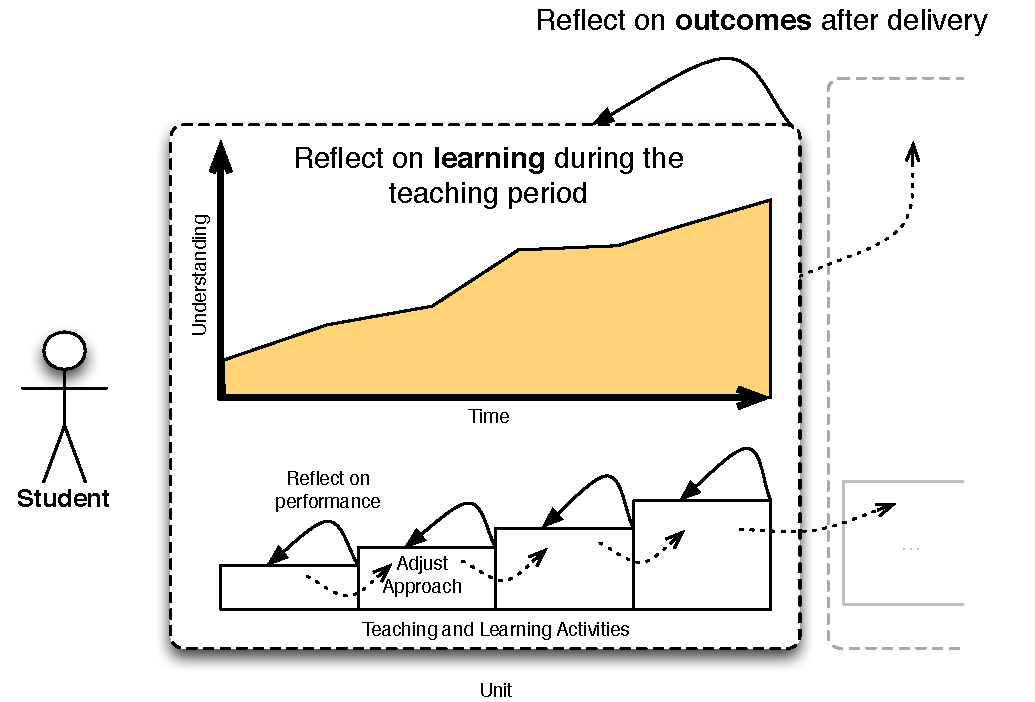
\includegraphics[width=\textwidth]{StudentReflection}
	\caption{Students relect on their learning during the teaching period, and on the outcomes they have achieved after the teaching period.}
	\label{fig:student_reflection}
\end{figure}

The role of reflection for students is shown in \fref{fig:student_reflection}. When each learning activity is concluded, students are encouraged to reflect on their learning. In this process students identify any areas they would like feedback on, and can use this to ensure their formative feedback is relevant to their current situation. By reflecting, and through the subsequent formative feedback, students reinforce the construction of the knowledge and are able to inform their actions for upcoming teaching and learning activities.

At the end of the teaching period for the unit, students are encouraged to reflect on their unit as a whole. Reflecting on their achievements, challenges overcome, work habbits and other aspects they felt influenced their learning. This process of reflection should help students consolidate their knowledge, drawing into clear focus exactly what they have achieved and, hopefully, ways they can improve their learning in future semesters.

\fref{fig:staff_reflection} shows the role of reflection for teaching staff. During the teaching period staff reflect upon the delivery of the teaching and learning activities and student progress. Common misconceptions identified in formative feedback can be used to update delivery during the teaching period. After the teaching period students' results, both in terms of grade distributions and quality of evidence demonstrated in the final summative assessment, can be drawn upon to suggest changes for subsequent unit deliveries. Reflections on teaching should be shared amongst all teaching staff related to the unit to encourage reflective practice, and to facilitate collaborative improvements.

\begin{figure}[ptbh]
	\centering
	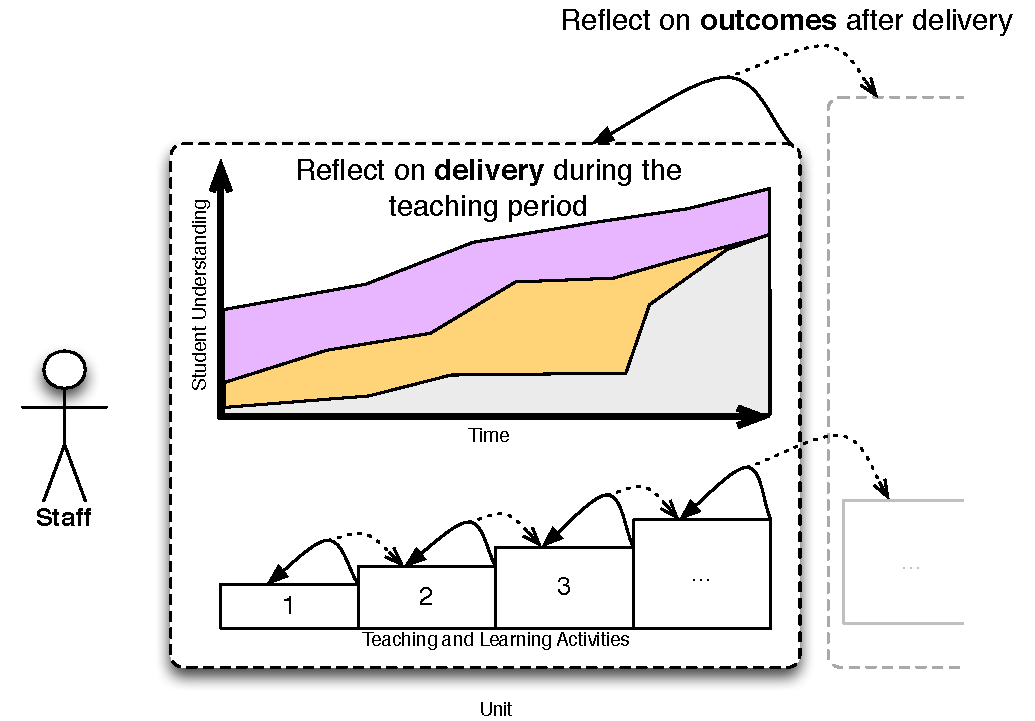
\includegraphics[width=\textwidth]{StaffReflection}
	\caption{Staff relect on delivery during the teaching period, and on the outcomes students achieved after the teaching period.}
	\label{fig:staff_reflection}
\end{figure} 

Reflection underpins all of the principles presented. Students engage in reflection as a tool to help them construct their knowledge, and the formative feedback enables student and staff reflections. Staff reflect on teaching and learning activities, their alignment to learning outcomes, and the depth and breadth of coverage. Reflections enable educators to realistically manage expectations of students, the support offered, and to help balance trust with mechanisms to avoid inappropriate behaviour. Even the very nature and composition of these principles have been the focus of ongoing reflective practice.

To ensure ongoing improvements for both students and staff, the model incorporates reflective practice across all aspects. Students engage in reflection throughtout the learning process, using their reflections to direct formative feedback and consolidate knowledge. Teaching staff reflect on delivery, progress, and outcomes to improve the teaching and learning environment to better meet student needs.

% subsection embed_reflective_practice_in_all_aspects (end)


\subsection{Be agile and willing to change} % (fold)
\label{ssub:be_agile_and_willing_to_change}

For reflective practice to actively enhance teaching educators must embrace change, focusing on aspects that will deliver the most value for students for the effort required. Similarly, as software developers this emphasis on delivering value by focusing on the things that matter most is reminiscent of the agile software development principles \cite{Martin:2003}. The agile software development community aimed to move away from heavyweight, documentation driven, software development processes toward a more \emph{agile} approach focused on outcomes. \citet{Beck:2001} documented the Agile Manifesto; the key priorities from a wide range of agile software development processes. The Agile Manifesto states: 

\begin{itemize}[noitemsep,nolistsep]
	\item \textbf{Individuals and interactions} \emph{over} processes and tools
	\item \textbf{Working software} \emph{over} comprehensive documentation
	\item \textbf{Customer collaboration} \emph{over} contract negotiation
	\item \textbf{Responding to change} \emph{over} following a plan
\end{itemize}

In many ways the evolution of software development process from the traditionally heavyweight processes to lightweight agile processes can be likened to a shift from a predominant Theory X environment to one which is predominantly Theory Y. The focus on documentation and rigid control over the development process is being relaxed, and developers are being trusted to deliver value. 

If we are to affect change in education from a mark driven Theory X environment, to a student centred Theory Y environment, then the agile software development principles provide useful guidance to inform our model. To realise all of the principles presented in this chapter it is necessary to adopt similar priorities in our teaching, valuing things that help students construct their knowledge over other less valuable activities.

To help manage change effectively we view the environment as consisting of an a) overall strategy, b) teaching and learning resources, and c) teaching and learning activities as shown in \fref{fig:strategy}. 

\begin{figure}[htbp]
	\centering
	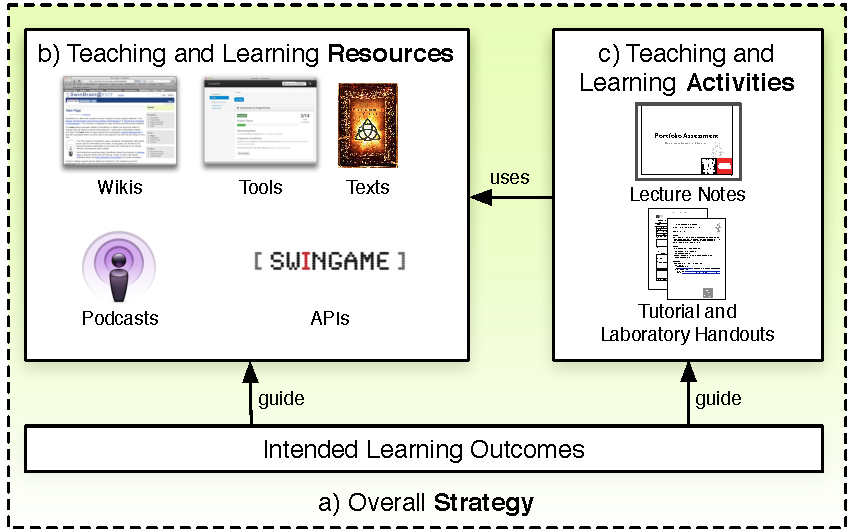
\includegraphics[width=0.85\textwidth]{StrategyResourcesActivities}
	\caption{Relationship between a) overall strategy, b) resources and c) activities used to manage change effectively.}
	\label{fig:strategy}
\end{figure}

The strategy for delivering unit content informs the choice of assessment strategy, approach to selecting unit content, and the development of the intended learning outcomes. The central role of the intended learning outcomes means that the overall strategy should not change unless significant issues are identified in the approach overall. Teaching and learning resources can then be separated from the teaching and learning activities. In this way we can create reusable resources that are independent of the activities that are used in, meaning that activities can be adjusted more freely to better help direct student efforts. The details of this approach are summarised in the following list.

%
% JG - I am not sure this is "details"...
%
% Do you flesh this out in a later chapter - if so could indicate this -or even forward ref
% and put there???
%
% It raises a lot of "how" questions which might be better deferred to with the answers later?
%


\begin{itemize}[noitemsep,nolistsep]
	\item Develop an overall \emph{strategy} for delivering the unit content. Then:
	\begin{itemize}[noitemsep,nolistsep]
		\item Select an appropriate assessment approach.
		\item Use principles about \emph{what} content should be covered to determine what content should be included in the unit.
		\item Derive intended learning outcomes from the approach selected to deliver content.
		\item Use the overall strategy to focus other teaching and learning resources and activities.
		\item Avoid changing strategy, unless approach has significant issues.
	\end{itemize}

	\item Create teaching and learning \emph{resources}.
	\begin{itemize}[noitemsep,nolistsep]
		\item Deliver material following the direction from the overall strategy.
		\item Make resources generic and self contained.
		\item See as providing a supporting role to the teaching and learning activities.
		\item Invest in initial development, actively reuse and enhance over time.
		\item Improve integration with delivery material as resources prove to be effective.
	\end{itemize}

	\item Design teaching and learning \emph{activities}.
	\begin{itemize}[noitemsep,nolistsep]
		\item Use these to focus student activity.
		\item Actively review each semester, and rework based on reflection.
	\end{itemize}
\end{itemize} 

% subsection be_agile_and_willing_to_change (end)


\subsection{Related Work on General Education Principles} % (fold)
\label{ssub:related_work_on_education_principles}

%
% JG - I am not sure about this section in terms of fit & content...
%
% Maybe could incorporate in the principles sections???
%
%


In discussing how to improve undergraduate education, \citet{Chickering:1987} listed seven principles for good practice in undergraduate education. These are practices that:
\begin{enumerate}[noitemsep,nolistsep]
	\item Encourages contact between students and faculty.
	\item Develops reciprocity and cooperation among students
	\item Encourages active learning
	\item Gives prompt feedback
	\item Emphasizes time on task
	\item Communicates high expectations
	\item Respects diverse talents and ways of learning
\end{enumerate}

The following list states how each of the principles from \citet{Chickering:1987} are integrated with the principles underlying this work. 
\begin{itemize}[noitemsep,nolistsep]
	\item The strong emphasis on frequent formative feedback should be used to help encourage contact between students and faculty. (\Pref{itm:formative}, \Pref{itm:support})
	\item This same formative process should also be harnessed to encourage sharing and cooperation amongst students. (\Pref{itm:formative},\Pref{itm:support},\Pref{itm:theory_y})
	\item The central nature of the students in constructing their knowledge necessitates an approach that encourages active learning. (\Pref{itm:construct},\Pref{itm:theory_y})
	\item The formative feedback process needs to ensure that work is returned promptly to students, ensuring they receive the feedback while it is still relevant. (\Pref{itm:formative})
	\item Communicating high expectations is included directly in our principles. (\Pref{itm:expectations})
	\item Assessment and teaching and learning activities need to be flexible, enabling different styles of learning and to engage with students diverse talents. (\Pref{itm:support})
\end{itemize}

% For outcomes based education, 

% \citet{Killen:2000} lists the 

% subsection related_work_on_education_principles (end)


\subsection{Summary} % (fold)
\label{ssub:summary_of_principles_on_how_to_teach}

This section presented the nine principles which guided decisions on how to teaching introductory programming. Each principle is backed by a range of education theories, and together the principles should enable the creation of an environment that is demanding but supportive, focused on students building knowledge, agile, constantly improving through reflections, and accepting of various individual strategies and pace of learning.

The next section details the principles related to \emph{what} we are going to teach.

% subsection summary_of_principles_on_how_to_teach (end)


% section principles_for_how_the_environment_should_operate (end)






\clearpage
\section{Principles to guide what we should teach} % (fold)
\label{sec:principles_to_guide_what_we_should_cover}

Principles specific to teaching introductory programming are presented in the following list. While the general principles helped shape the overall teaching and learning environment, these principles helped shape specifics in the curriculum, activities, and assessment tasks.
\begin{itemize}[noitemsep,nolistsep]
	\item Set the strategy, and structure learning, around a programming paradigm. (\Pref{itm:paradigm})
	\item Focus on programming concepts \emph{over} language syntax. (\Pref{itm:concepts})
	\item Use programming languages as they were designed to be used. (\Pref{itm:authentic})
	% \item Program code is not, by itself, a suitable means of measuring learning outcomes.
\end{itemize}


%
% JG - I suggest summarise the items from the subsections briefly here
%


Each of these principles is expanded upon in the following sections, and linked to associated research.


\subsection{Set the strategy and structure learning around programming a paradigm} % (fold)
\label{ssub:strategy_around_paradigm}

The programming paradigm chosen for introductory programming can have a large impact on the way the unit is taught and, therefore, the unit's intended learning outcomes. To endeavour that the foundations of a unit do not need to change, a programming paradigm, such as the procedural, functional or object oriented paradigm, needs to be chosen.This will then form the core of the overall strategy for the unit.

Which programming paradigm should be taught first is a popular topic in computing education research. The following list indicates the range of approaches from imperative-first to objects-first approaches.
\begin{itemize}[noitemsep,nolistsep]
	\item Imperative programming first such as with \citet{Koffman:1988a}.
	\item \citet{Cooper:2003} suggest a course working with graphics prior to introductory programming to help students with problem solving skills.
	\item \citet{Felleisen:2004} described a approaching to teaching introductory programming using the functional paradigm and the Scheme programming language.
	\item \citet{Howe:2004} presented a components-first approach.
	\item \citet{Bennedsen:2004} argued for the use of a model-first approach using the object oriented programming paradigm.
\end{itemize}

 With the predominant role of objects in industry, a common trend has been to move from imperative-first approaches to objects-first approaches. This approach has ``failed'' according to \citet{Astrachan:2005} and \citet{Reges:2006}. While \citet{Ehlert:2009} reported no significant difference between approaches using objects-first and objects-later, their later work \cite{Ehlert:2010} indicated the objects-later approach had a greater comfort level for students. \citet{Robins:2003} include the imperative-first and objects-first approaches as one of their four themes from the literature on learning and teaching introductory programming. \citet{Lister:2006a} provide an in depth look at the research perspectives on the topic of objects-first, but in general there is no consensus on which approach should be taken.

The design of the introductory programming units developed in this research work there was a need to choose which \emph{x}-first approach will be used. The main decision seemed to be between the imperative-first, objects-first or functional-first approaches. Whichever approach is taken, the choices guide which concepts are covered in the unit and the order in which these can be tackled.

% subsection set_the_strategy_and_structure_learning_around_programming_a_paradigm (end)

\subsection{Focus on programming concepts} % (fold)
\label{sub:focus_on_programming_concepts}

There are various views of programming in the literature. On perspective views programming from a mathematical basis \cite{Denning:1989,Dijkstra:1989,Hoare:1969}, others see it as an exercise in problem solving \cite{Palumbo:1990}, modelling concepts \cite{Bennedsen:2004}, though most textbooks approach the topic through language syntax and features \cite{Robins:2003}. In this work we avoided the standard textbook approach, and instead we focused on programming concepts.

A similar idea was expressed in \citet{Goldman:2004} as a \emph{concept based} approach. The work introduced students to a number of ``big ideas'' related to software development using the JPie interactive programming environment. Our approach differs in that we focus on the ``small ideas'' that programs are build upon. In this way we build depth across these ideas rather than breadth, in line with our general principles.

Topics such as variables, procedures, control flow, etcetera are each approached as a concept. This is similar to the model-based approach of \citet{Bennedsen:2004}, but applied to procedural programming concepts. By focusing on concepts we aim to provide students with reasons why the various programming features should be used, when different abstractions should be used, and help students develop means of understanding these abstract ideas. This concept based approach can be applied to procedural programming concepts, object oriented programming concepts, and other programming paradigms.

Winslow's comparison study of expert and novice programmers \cite{Winslow:1996} indicated that expert programmers tend to ``abstract from a particular language to the general concept''. By focusing on the concepts first we hope to instil similar expert-like ideas in the students. Students are encouraged to create \emph{conceptual programs}, which can then be mapped to code using the programming language syntax rules. Focusing first on the concepts should encourage a depth of understanding, with students going beyond surface learning of the syntax used and thinking conceptually about what they are trying to achieve.

Programming concepts are tightly interrelated, and yet there is a need to provide a sequence of activities that can be introduced to students without overloading them initially. In designing these activities we aimed to ensure that concepts could be introduced to students in such a way as to reduce the amount of ``magic'' to a minimum. Limiting the cases where students had to do something without being able to reason why with the concepts covered so far.

The aim of this is to enable students to explore language features. At each stage in the process students should have sufficient concepts to be able to understand the programs they are asked to create. To extend students further they can be asked to experiment with features, using the concepts covered to create programs they are interested in. Ideally this would enhance student motivation, and ensure they spend sufficient time on the task.

The focus on programming concepts means there is a need to: %also in supporting chapter
\begin{itemize}[noitemsep,nolistsep]
	\item Introduce programming concepts incrementally;
	\item Provide students with time to put concepts into practice;
	\item See syntax as a means to an end, not an end in itself;
	\item Avoid using language features before concepts that can explain their use; and
	\item Map concepts to code using programming language grammars.
\end{itemize} 

% section principles_to_guide_what_we_should_cover (end)

\subsection{Use programming languages as they were designed to be used} % (fold)
\label{ssub:use_programming_languages_as_they_were_designed_to_be_used}

While we agree with the ``back to basics'' approach of \citet{Reges:2006}, we want to emphasise using programming languages in the way they were designed to be used. Our emphasis on programming concepts has deliberately relegated language to a secondary role, and one that can be changed by learning new syntax rules. Given this, changing between languages is less problematic, and therefore we should not use a language for its industry relevance. Rather, language choice should be based on the programming concepts it supports, its available across computing platforms, and the level of support it offers novices.

Programming language choice for introductory programming is as popular in the Computing Education Research literature as the choice of programming paradigm. The following list covers a select number of well-cited papers on which programming language to use in teaching introductory programming, ordered by year it shows the shift from procedural languages to object oriented languages.

%
% JG - I suggest rethink the use of this long list approach
%



\begin{itemize}[noitemsep,nolistsep]
	\item \citet{Koffman:1988} argued for Modula-2 over Pascal, PL/1 and Ada, 
	\item \citet{Mody:1991} argued against C, and C++ for its lack of coherence, simplicity, understandability and implementability. 

	\item \citet{Roberts:1993} discusses Stanford's shift from Pascal to C, addressing common issues with C by providing libraries to encapsulate complex features, emphasising procedural and modular abstractions, and focusing on the discipline of software engineering.

	\item \citet{Brilliant:1996} discussed programming paradigm and language selection for introductory programming. They concluded that there was no clear advantage to starting with either procedural programming, object-oriented programming, or functional programming paradigms. In terms of language they discussed moving from Pascal to Ada, C, C++, or Scheme.

	\item \citet{Boszormenyi:1998} argued for Modula-3 over Java, discussing features that are useful to be taught in introductory programming yet missing from Java.

	\item \citet{Howell:2003} claimed that through structured labs, comprehensive grade sheets, in-class grading and frequent feedback any programming language could be used.

	\item \citet{Gupta:2004} suggested that a first language should strike a balance between being easy to grasp and supporting advanced concepts needed for later units.

	\item \citet{Kelleher:2005} provided a detailed examination of a wide range of programming languages used for teaching introductory programming. Their work discussed various efforts to help make programming more accessible for novices, including systems that range in support from look at the way programs are expressed, how programs are structured, understanding of program execution, to systems that embed learning support. While the work reported on a range of systems it does not provide any recommendations on which language to use.

	\item \citet{Bishop:2006} presented the pros and cons, from their experiences, in using the C\# programming language, and provided some recommendations for those looking at using the language.

	\item \citet{Mannila:2006} argued for the use of Python due to its simplicity, with examples comparing Python to Java.

	\item \citet{Mannila:2006a} provided a set of criteria for comparing language features for introductory programming. The study then compared several languages, with Eiffel, Java and Python achieving the highest scores.

	\item \citet{Pendergast:2006} provided a reflection on teaching introductory programming with Java over a number of years, highlighting some of the issues encountered and mechanisms to avoid these.

	\item \citet{Maloney:2010} described the Scratch programming environment, a visual programming language designed primarily for students aged between 8 and 16.

	\item \citet{Anik:2011} used the Analytic Network Process methodology to help guide the decision of which language should be used first. The relative weightings given to the various aspects resulted in Java being ranked above the other languages.
\end{itemize}

Interestingly, underlying many of these papers is the idea that switching language is difficult. For example, \citet{Brilliant:1996} indicated that teaching multiple languages increases the overhead necessary to cover language details and peculiarities. By having a focus on programming concepts over language syntax this work aimed to tackle this problem from a different angle. In our previous teaching we noticed that students tended to focus on or ``cling'' to syntax. Shifting language was a major effort as it was syntax they had learnt. Students felt they were ``Java programmers'' or ``C/C++ programmers''; they did not see that they were learning something far more important, they were not learning a specific language, they were learning to program. 

This focus also becomes evident when you examine the title of many introductory programming units. Introductory programming unit titles like ``Introduction to Programming with C'' and ``Software Development in Java'' give the impression that the language is important, raising its role from supportive to central in the unit.

%
% JG - again, perhaps "was" -> "is guided by" - I assume OTHERS could chose diff langs but still fulfil the principles??
% 
% 
% 


Choosing a language for the \emph{concept-based} approach to introductory programming was guided by the following principles:
\begin{itemize}[nolistsep,noitemsep]
	\item \textbf{Focus on programming concepts} \emph{over} language syntax.
	%Remember we are not teaching a language, we are teaching students to program.
	\item \textbf{Teach students to learn the language} \emph{over} teaching the language explicitly.
	%Do not teach the language explicitly, teach students to learn languages themselves.
	\item \textbf{Value languages that support the concepts to be learnt} \emph{over} the languages that are the current industry trend.
	%Choose a language, or languages, that support the concepts that need to be covered.
	\item \textbf{Use languages that support multiple operating systems} \emph{over} those tied tightly to a single platform. 
	%Ensure support for multiple operating systems, enabling students to use their preferred platform.
	\item \textbf{See multiple languages as an important part of the learning} \emph{over} focusing on a single language.
	%See multiple languages as an important part of the learning, not an unnecessary overhead.
	\begin{itemize}
		\item Use multiple languages to encourage students to focus on concepts over programming language syntax.
		\item Expose students to language differences enabling them to see different strengths and weaknesses. 
		\item Encourage students to see that they are learning to program, not learning one programming language.
		\item Foster the attitude that language is a choice, students should not feel constrained to one language and should be open to possibilities other languages offer.
	\end{itemize}
\end{itemize}

As with the Agile Manifesto, we agree that there is value in the items on the right, but we value the items on the left more.

One aspect that is different from other work is the importance of the use of the language in industry. If the concept based approach is successful students will be able to quickly develop skills in industry relevant languages in later units. The first units can focus on using languages that best meet educational requirements, while later units can cover language specific details and peculiarities briefly knowing students have an understanding of underlying concepts and the ability to learning new languages themselves. 

% \cite{Koffman:1988,Roberts:1993,Brilliant:1996}
% Arguments against Pascal 
% \begin{enumerate}
% 	\item Missing language features such as open arrays, function pointers, and string manipulation.
% 	\item Not widely used beyond introductory programming.
% 	\item Lack of data abstraction and information hiding.
% \end{enumerate}


% subsection use_programming_languages_as_they_were_designed_to_be_used_ (end)


\subsection{Summary} % (fold)
\label{ssub:summary_of_principles_for_what_to_teach}

This section proposed the use of a \emph{concept-based} approach to teaching introductory programming. This approach focuses on teaching programming concepts directly, with use of the programming language grammars to help students map concepts to code. The aim of this approach is to help students focus on the concepts, while providing them with tools they can use to learn any relevant programming language. The expected outcome of this approach is that programming language choice is much less important than which programming paradigm choice. 

% subsection summary_of_principles_for_what_to_teach (end)

\clearpage
\section{Summary of Guiding Principles} % (fold)
\label{sec:summary_of_guiding_principles}

This chapter outlined twelve principles related to both \emph{how} and \emph{what} we aim to teach in our constructively aligned introductory programming.
\begin{itemize}[noitemsep,nolistsep]
	\item Nine principles describe \emph{how} the teaching and learning environment should operate:
	\begin{enumerate}[noitemsep,nolistsep]
		\item \label{itm:construct} Recognise that students construct knowledge in response to activity.
		\item \label{itm:align} Align activities and assessment to intended learning outcomes.
		\item \label{itm:formative} Assess learning outcomes, not learning pace or product outcomes.
		\item \label{itm:depth} Focus on depth of understanding over breadth of coverage.
		\item \label{itm:expectations} Communicate high expectations.
		\item \label{itm:support} Actively support student efforts.
		\item \label{itm:theory_y} Trust and empower students to manage their own learning.
		\item \label{itm:agile} Be agile and willing to change in response to measurable indicators.
		\item \label{itm:reflect} Embed reflective practice in all aspects.
	\end{enumerate}
	\item Three principles help guide \emph{what} we aim to teach:
	\begin{enumerate}[start=10,noitemsep,nolistsep]
		\item \label{itm:paradigm} Set the strategy and structure learning around a programming paradigm.
		\item \label{itm:concepts} Focus on programming concepts, not language syntax.
		\item \label{itm:authentic} Use programming languages as they were designed to be used.
		% \item Program code is not, by itself, a suitable means of measuring learning outcomes.
	\end{enumerate}
\end{itemize}

\cref{cha:approach} will outline a model for constructively aligned introductory programming units. The model presented was created through the application of these principles, and the model's ability to embody these principles is discussed.

% section summary_of_guiding_principles (end)

% chapter guiding_principles (end)